\documentclass[12pt]{article}
\usepackage{amsmath}
\usepackage{graphicx}
\usepackage{hyperref}
\usepackage[utf8]{inputenc}
\usepackage{geometry}
\usepackage{mathtools}
\usepackage{empheq}
\usepackage{listings}
\usepackage{xcolor}
\usepackage{minted}
\usepackage{svg}


\definecolor{LightGray}{gray}{0.9}

\graphicspath{ {./assets/} }
\geometry{margin=0.6in}

\title{CHEN 461 HW 5}
\author{Mark Levchenko}
\date{January 2023}

\begin{document}


\begin{enumerate}

% Problem 1 %%%%%%%%%%%%%%%%%%%%%%%%%%%%%%%%%%%%%%%%%%%%%%%%%%%%%%%%%%%%%%%%%%%%%%%%%%%
\newpage
\item Problem 4.8
\begin{enumerate}
    \item 
    \begin{align*}
        Y_1(s) &= \frac{k_1}{\tau_1 s + 1} U(s) \\
        Y_2(s) &= \frac{-k_2}{\tau_2 s + 1} U(s) \\
        Y(s) &= \left(\frac{k_1}{\tau_1 s + 1} - \frac{k_2}{\tau_2 s + 1}\right) U(s) \\
        U(s) &= \frac{M}{s} \\
        \intertext{Linear combination}
        \Aboxed{y(t) &= k_1 M \left(1 - e^{-t/\tau_1}\right) - k_2 M \left(1 - e^{-t/\tau_2}\right)} \\
        \frac{dy}{dt} &= \frac{k_1 M}{\tau_1} e^{-t/\tau_1} - \frac{k_2 M}{\tau_2} e^{-t/\tau_2} \\
        \Aboxed{\frac{dy}{dt}(0) &= \frac{k_1 M}{\tau_1} - \frac{k_2 M}{\tau_2} }\\
        \intertext{As $t\rightarrow\infty$}
        \Aboxed{y(t) &= \frac{k_1 M}{\tau_1} - \frac{k_2 M}{\tau_2}}
    \end{align*}
    \item Plot:

    \includesvg{461HW5_P48b.svg}

    Initially, the second block's output is larger than the first block's output. As a result, the second block's output pulls the combined output negative. The first output eventually outpaces the second output, and the output reaches a new higher steady state.
    
    \item Plot:

    \includesvg{461HW5_P48c.svg}

    A similar situation to that of part b occurs in part c. Except, the first output is initially larger than the second output. The combined output reaches a peak before the second output matches the first output and pulls the combined output to a new steady state, lower than the peak but higher than the initial.
    
\end{enumerate}

Plotting code:

\begin{minted}[
framesep=2mm,
baselinestretch=1.2,
bgcolor=LightGray,
fontsize=\footnotesize,
breaklines,
]{python}
import numpy as np
import matplotlib.pyplot as plt

k_1 = 2
tau_1 = 4
k_2 = 1
tau_2 = 1
M = 1

func = lambda t: k_1 * M * (1 - np.exp(-t / tau_1)) - k_2 * M * (1 - np.exp(-t / tau_2))

t_ran = np.linspace(0, 20, 100)
plt.plot(t_ran, func(t_ran))
plt.xlabel(r"t")
plt.ylabel(r"y(t)")
plt.title("Problem 4.8b Response Plot")

k_1 = 2
tau_1 = 1/4
k_2 = 1
tau_2 = 1
M = 1

func = lambda t: k_1 * M * (1 - np.exp(-t / tau_1)) - k_2 * M * (1 - np.exp(-t / tau_2))

t_ran = np.linspace(0, 5, 100)
plt.plot(t_ran, func(t_ran))
plt.xlabel(r"t")
plt.ylabel(r"y(t)")
plt.title("Problem 4.8c Response Plot")
\end{minted}

% Problem 2 %%%%%%%%%%%%%%%%%%%%%%%%%%%%%%%%%%%%%%%%%%%%%%%%%%%%%%%%%%%%%%%%%%%%%%%%%%%
\newpage
\item Problem 2

Calculate the overall transfer function of the system represented by the following block
diagram:

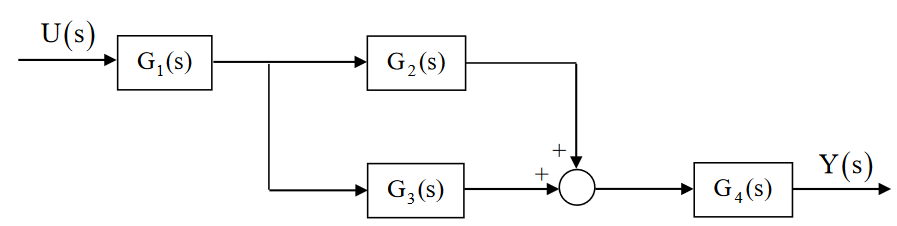
\includegraphics[scale=0.8]{p2.png}

\begin{align*}
    Y_1(s) &= G_1(s) U(s) \\
    Y_2(s) &= (G_2(s) + G_3(s)) U_2(s) \\
    Y_2(s) &= \left(G_2(s) + G_3(s)\right) G_1(s) U(s) \\
    Y(s) &= G_4(s) U_3(s) \\
    Y(s) &= G_4(s) \left(G_2(s) + G_3(s)\right) G_1(s) U(s) \\
    \Aboxed{Y(s) &= \left(G_2(s) + G_3(s)\right) G_1(s) G_4(s) U(s)}
\end{align*}


% Problem 3 %%%%%%%%%%%%%%%%%%%%%%%%%%%%%%%%%%%%%%%%%%%%%%%%%%%%%%%%%%%%%%%%%%%%%%%%%%%
\newpage
\item Problem 5.8
\begin{align*}
    kM &\approx 38 \\
    A \approx 47 - 38 &= 9 \\
    \frac{A}{kM} &= \exp{\left(-\frac{\pi\zeta}{\sqrt{1 - \zeta^2}}\right)} \\
    \frac{9}{38} &= \exp{\left(-\frac{\pi\zeta}{\sqrt{1 - \zeta^2}}\right)} \\
    \Aboxed{\zeta &= 0.4168} \\
    T &\approx 20 \\
    T &= \frac{2\pi\tau}{\sqrt{1 - \zeta^2}} \\
    20 &= \frac{2\pi\tau}{\sqrt{1 - 0.4168^2}} \\
    \Aboxed{\tau &= 2.893} \\
    M = 0.5 \cdot 76 &= 38 \\
    \Aboxed{k &= 1}
\end{align*}

% Problem 4 %%%%%%%%%%%%%%%%%%%%%%%%%%%%%%%%%%%%%%%%%%%%%%%%%%%%%%%%%%%%%%%%%%%%%%%%%%%
\newpage
\item Problem 4.2
Additional Question:

For the reaction scheme of question d), suppose that F/V = 0.5, k1 = 3, k–1 = 1.25, k2 = 0.75.

→ Put your model in matrix form, i.e. in the form of Eqns. (5.6.3) and (5.6.4), using deviation variables

→ Use the Control Systems Toolbox of MATLAB to:

• calculate and plot the response to a unit step change in Cin,R and to a unit impulse change in Cin,R

• calculate the transfer function

• calculate and plot the unit step response and unit impulse response based on the transfer function

\begin{enumerate}
    \item 
    \begin{align*}
        V \frac{dC_R}{dt} &= F C_{in,R} - F C_R - V k_1 C_R \\
        V \frac{dC_P}{dt} &= V k_1 C_R - F C_P - V k_2 C_P
    \end{align*}
    
    
    \item
    \begin{align*}
        V C_R(s) s &= F C_{in,R}(s) - F C_R(s) - Vk_1C_R(s) \\
        C_R(s) &= \frac{F}{Vs + F + Vk_1} C_{in,R}(s) \\
        V C_P(s) s &= V k_1 C_R(s) - F C_P(s) - V k_2 C_P(s) \\
        C_P(s) (V s + F + V k_2) &= V k_1 C_R(s) \\
        C_P(s) (V s + F + V k_2) &= \frac{F V k_1}{Vs + F + Vk_1} C_{in,R}(s) \\
        C_P(s) &= \frac{F V k_1}{(Vs + F + Vk_1) (V s + F + V k_2)} C_{in,R}(s) \\
        G(s) &= \frac{F V k_1}{(Vs + F + Vk_1) (V s + F + V k_2)} \\
        G(s) &= \frac{F V k_1}{V^2s^2 + 2FVs + V^2sk_2 + F^2 + FVk_2 + V^2k_1s + FVk_1 + V^2k_1k_2} \\
        G(s) &= \frac{F V k_1}{V^2s^2 + s (2FV + V^2k_2 + V^2k_1) + F^2 + FVk_2 + FVk_1 + V^2k_1k_2} \\
        G(s) &= \frac{\frac{V}{F} k_1}{\left(\frac{V}{F}\right)^2 s^2 + s \left(2\frac{V}{F} + \left(\frac{V}{F}\right)^2 (k_2 + k_1)\right) + \left(\frac{V}{F}\right)^2 + \frac{F}{V} (k_2 + k_1) + \left(\frac{V}{F}\right)^2 k_1k_2} \\
        G(s) &= \frac{\frac{V}{F} k_1}{\left(\frac{V}{F}\right)^2 s^2 + s \left(2\frac{V}{F} + \left(\frac{V}{F}\right)^2 (k_2 + k_1)\right) + \left(\frac{V}{F} + k_1\right) \left(\frac{V}{F} + k_2\right)}
    \end{align*}

    \item
    \begin{align*}
        G(s) &= \frac{k}{\tau^2 s^2 + 2 \zeta \tau s + 1} \\
        k &= \frac{\frac{V}{F} k_1}{\left(\frac{V}{F} + k_1\right) \left(\frac{V}{F} + k_2\right)} \\
        \tau &= \sqrt{\frac{\left(\frac{V}{F}\right)^2}{\left(\frac{V}{F} + k_1\right) \left(\frac{V}{F} + k_2\right)}} \\
        2\tau\zeta &= \frac{\left(2\frac{V}{F} + \left(\frac{V}{F}\right)^2 (k_2 + k_1)\right)}{\left(\frac{V}{F} + k_1\right) \left(\frac{V}{F} + k_2\right)} \\
        2\tau\zeta &= \frac{\left(2\frac{V}{F} + \left(\frac{V}{F}\right)^2 (k_2 + k_1)\right)}{\sqrt{\left(\left(\frac{V}{F} + k_1\right) \left(\frac{V}{F} + k_2\right)\right)^2}} \\
        2\zeta \frac{V}{F} &= \frac{\left(2\frac{V}{F} + \left(\frac{V}{F}\right)^2 (k_2 + k_1)\right)}{\sqrt{\left(\frac{V}{F} + k_1\right) \left(\frac{V}{F} + k_2\right)}} \\
        \zeta &= \frac{1 + \frac{V}{2F} (k_2 + k_1)}{\sqrt{\left(\frac{V}{F} + k_1\right) \left(\frac{V}{F} + k_2\right)}} \\
        \tau &= \frac{\frac{V}{F}}{\sqrt{\left(\frac{V}{F} + k_1\right) \left(\frac{V}{F} + k_2\right)}}
    \end{align*}

    \item

    Reversible

    State Space:
    \begin{align*}
        V \frac{dC_R}{dt} &= F C_{in,R} - F C_R - V k_1 C_R + V k_{-1} C_P \\
        V \frac{dC_P}{dt} &= V k_1 C_R - F C_P - V k_2 C_P - V k_{-1} C_P
    \end{align*}

    Transfer Function:

    \begin{align*}
        V s C_R(s) &= F C_{in,R}(s) - C_R(s) (F + V k_1) + V k_{-1} C_P(s) \\
        C_R(s) (V s + F + V k_1) &= F C_{in,R}(s) + V k_{-1} C_P(s) \\
        C_R(s) &= \frac{F}{V s + F + V k_1} C_{in,R}(s) + \frac{V k_{-1}}{V s + F + V k_1} C_P(s) \\
        V s C_P(s) &= V k_1 C_R(s) - F C_P(s) - V k_2 C_P(s) - V k_{-1} C_P \\
        C_P(s) (V s + F + V k_2 + V k_{-1}) &= V k_1 C_R(s) \\
        C_P(s) (V s + F + V k_2 + V k_{-1}) &= \frac{F V k_1}{V s + F + V k_1} C_{in,R}(s) + \frac{V^2 k_{-1} k_1}{V s + F + V k_1} C_P(s) \\
        \frac{F V k_1}{V s + F + V k_1} C_{in,R}(s) &= C_P(s) \left((V s + F + V k_2 + V k_{-1}) - \frac{V^2 k_{-1} k_1}{V s + F + V k_1}\right) \\
        (F V k_1) C_{in,R}(s) &= C_P(s) \left((V s + F + V k_2 + V k_{-1}) (V s + F + V k_1) - V^2 k_{-1} k_1\right)
    \end{align*}
    \begin{align*}
        C_P(s) &= C_{in,R}(s) \frac{F V k_1}{V^2 s^2 + s (2 F V + V^2 (k_1 + k_2 + k_{-1})) + (F^2 + F V (k_1 + k_2 + k_{-1}) + V^2 k_1 k_2)} \\
        G(s) &= \frac{F V k_1}{V^2 s^2 + s (2 F V + V^2 (k_1 + k_2 + k_{-1})) + (F^2 + F V (k_1 + k_2 + k_{-1}) + V^2 k_1 k_2)}
    \end{align*}

    % \[
    %     V^2 s^2 + s (2 F V + V^2 (k_1 + k_2 + k_{-1})) + (F^2 + F V (k_1 + k_2 + k_{-1}) + V^2 k_1 k_2 + V^2 k_{-1} k_1)
    % \]

    % \[
    %     V^2 s^2 + s (2 F V + V^2 (k_1 + k_2 + k_{-1})) + (F^2 + F V (k_1 + k_2 + k_{-1}) + V^2 k_1 k_2)
    % \]


    \item[(Matlab)]
    \begin{align*}
        V \frac{dC_R}{dt} &= F C_{in,R} - F C_R - V k_1 C_R + V k_{-1} C_P \\
        V \frac{dC_P}{dt} &= V k_1 C_R - F C_P - V k_2 C_P - V k_{-1} C_P \\
        \frac{dC_R}{dt} &= \frac{F}{V} C_{in,R} - \frac{F}{V} C_R - k_1 C_R + k_{-1} C_P \\
        \frac{dC_P}{dt} &= k_1 C_R - \frac{F}{V} C_P - k_2 C_P - k_{-1} C_P \\
        \frac{dx_1}{dt} &= a_{11} x_1 + a_{12} x_2 + b_1 u \\
        \frac{dx_2}{dt} &= a_{21} x_1 + a_{22} x_2 + b_2 u \\
        y &= c_1 x_1 + c_2 x_2 + du \\
        \frac{dC_R}{dt} &= - \left(\frac{F}{V} + k_1\right) C_R + k_{-1} C_P + \frac{F}{V} C_{in,R} \\
        \frac{dC_P}{dt} &= -\left(\frac{F}{V} + k_2 + k_{-1}\right) C_P + k_1 C_R \\
        C_P &= C_P \\
        \frac{d}{dt}\begin{bmatrix}
        C_R \\
        C_P \\
        \end{bmatrix} &= \begin{bmatrix}
        - \left(\frac{F}{V} + k_1\right) & k_{-1} \\
        k_1 & -\left(\frac{F}{V} + k_2 + k_{-1}\right) \\
        \end{bmatrix} \begin{bmatrix}
        C_R \\
        C_P \\
        \end{bmatrix} + \begin{bmatrix}
        \frac{F}{V} \\
        0 \\
        \end{bmatrix} C_{in,R} \\
        C_P &= \begin{bmatrix}
        0 & 1 \\
        \end{bmatrix} \begin{bmatrix}
        C_R \\
        C_P \\
        \end{bmatrix} + 0 \cdot du \\
        \frac{F}{V} &= 0.5 \\
        k_1 &= 3 \\
        k_{-1} &= 1.25 \\
        k_2 &= 0.75
    \end{align*}

    Response plot:

    \includesvg{461HW5_P4.svg}

    Response plot from manual transfer function:

    \includesvg{461HW5_P4_manual.svg}

    Transfer function output:

    TransferFunctionContinuous(
    array([1.5]),
    array([1., 6., 5.]),
    dt: None
    )

    \[
        G(s) = \frac{1.5}{s^2 + 6s + 5}
    \]

Code for solving the system

\begin{minted}[
framesep=2mm,
baselinestretch=1.2,
bgcolor=LightGray,
fontsize=\footnotesize,
breaklines,
]{python}
import numpy as np
import matplotlib.pyplot as plt
import scipy.signal as signal

# constants
F_V = 0.5
k_1 = 3
k_b = 1.25
k_2 = 0.75

# matrices
A = np.array([
    [-(F_V + k_1), k_b],
    [k_1, -(F_V + k_2 + k_b)]
])
B = np.array([
    [F_V],
    [0]
])
C = np.array([0, 1])
D = 0

# define state space system
sys = signal.StateSpace(A, B, C, D)

# compute step/impulse response
t_step, y_step = sys.step()

t_impulse, y_impulse = sys.impulse()

# plot
plt.plot(t_step, y_step, label="Step response")
plt.plot(t_impulse, y_impulse, label="Impulse response")
plt.xlabel(r"t")
plt.ylabel(r"y(t)")
plt.title("Problem 4.2 CSTR with Reversible Reaction Response")
plt.legend()

# compute transfer function
transfer_func = sys.to_tf()

print(transfer_func)

# manually create system from transfer function
sys_manual = signal.lti(transfer_func.num, transfer_func.den)

# comput step/impulse response
t_step, y_step = sys_manual.step()

t_impulse, y_impulse = sys_manual.impulse()

plt.plot(t_step, y_step, label="Step response")
plt.plot(t_impulse, y_impulse, label="Impulse response")
plt.xlabel(r"t")
plt.ylabel(r"y(t)")
plt.title("Problem 4.2 CSTR with Reversible Reaction Response")
plt.legend()
\end{minted}
\end{enumerate}



\end{enumerate}
\end{document}